\documentclass[12pt,letterpaper,fleqn]{hmcpset}
\usepackage[margin=1in]{geometry}
\usepackage{graphicx}
\usepackage{amsmath,amssymb}
\usepackage{enumerate}
\usepackage{hyperref}
\usepackage{parskip}

% Theorems
\usepackage{amsthm}
\renewcommand\qedsymbol{$\blacksquare$}
\makeatletter
\@ifclassloaded{article}{
    \newtheorem{definition}{Definition}[section]
    \newtheorem{example}{Example}[section]
    \newtheorem{theorem}{Theorem}[section]
    \newtheorem{corollary}{Corollary}[theorem]
    \newtheorem{lemma}{Lemma}[theorem]
}{
}
\makeatother

% Random Stuff
\setlength\unitlength{1mm}

\newcommand{\insertfig}[3]{
\begin{figure}[htbp]\begin{center}\begin{picture}(120,90)
\put(0,-5){\includegraphics[width=12cm,height=9cm,clip=]{#1.eps}}\end{picture}\end{center}
\caption{#2}\label{#3}\end{figure}}

\newcommand{\insertxfig}[4]{
\begin{figure}[htbp]
\begin{center}
\leavevmode \centerline{\resizebox{#4\textwidth}{!}{\input
#1.pstex_t}}
\caption{#2} \label{#3}
\end{center}
\end{figure}}

\long\def\comment#1{}

\newcommand\norm[1]{\left\lVert#1\right\rVert}
\DeclareMathOperator*{\argmin}{arg\,min}
\DeclareMathOperator*{\argmax}{arg\,max}

% bb font symbols
\newfont{\bbb}{msbm10 scaled 700}
\newcommand{\CCC}{\mbox{\bbb C}}

\newfont{\bbf}{msbm10 scaled 1100}
\newcommand{\CC}{\mbox{\bbf C}}
\newcommand{\PP}{\mbox{\bbf P}}
\newcommand{\RR}{\mbox{\bbf R}}
\newcommand{\QQ}{\mbox{\bbf Q}}
\newcommand{\ZZ}{\mbox{\bbf Z}}
\renewcommand{\SS}{\mbox{\bbf S}}
\newcommand{\FF}{\mbox{\bbf F}}
\newcommand{\GG}{\mbox{\bbf G}}
\newcommand{\EE}{\mbox{\bbf E}}
\newcommand{\NN}{\mbox{\bbf N}}
\newcommand{\KK}{\mbox{\bbf K}}
\newcommand{\KL}{\mbox{\bbf KL}}

% Vectors
\renewcommand{\aa}{{\bf a}}
\newcommand{\bb}{{\bf b}}
\newcommand{\cc}{{\bf c}}
\newcommand{\dd}{{\bf d}}
\newcommand{\ee}{{\bf e}}
\newcommand{\ff}{{\bf f}}
\renewcommand{\gg}{{\bf g}}
\newcommand{\hh}{{\bf h}}
\newcommand{\ii}{{\bf i}}
\newcommand{\jj}{{\bf j}}
\newcommand{\kk}{{\bf k}}
\renewcommand{\ll}{{\bf l}}
\newcommand{\mm}{{\bf m}}
\newcommand{\nn}{{\bf n}}
\newcommand{\oo}{{\bf o}}
\newcommand{\pp}{{\bf p}}
\newcommand{\qq}{{\bf q}}
\newcommand{\rr}{{\bf r}}
\renewcommand{\ss}{{\bf s}}
\renewcommand{\tt}{{\bf t}}
\newcommand{\uu}{{\bf u}}
\newcommand{\ww}{{\bf w}}
\newcommand{\vv}{{\bf v}}
\newcommand{\xx}{{\bf x}}
\newcommand{\yy}{{\bf y}}
\newcommand{\zz}{{\bf z}}
\newcommand{\0}{{\bf 0}}
\newcommand{\1}{{\bf 1}}

% Matrices
\newcommand{\Ab}{{\bf A}}
\newcommand{\Bb}{{\bf B}}
\newcommand{\Cb}{{\bf C}}
\newcommand{\Db}{{\bf D}}
\newcommand{\Eb}{{\bf E}}
\newcommand{\Fb}{{\bf F}}
\newcommand{\Gb}{{\bf G}}
\newcommand{\Hb}{{\bf H}}
\newcommand{\Ib}{{\bf I}}
\newcommand{\Jb}{{\bf J}}
\newcommand{\Kb}{{\bf K}}
\newcommand{\Lb}{{\bf L}}
\newcommand{\Mb}{{\bf M}}
\newcommand{\Nb}{{\bf N}}
\newcommand{\Ob}{{\bf O}}
\newcommand{\Pb}{{\bf P}}
\newcommand{\Qb}{{\bf Q}}
\newcommand{\Rb}{{\bf R}}
\newcommand{\Sb}{{\bf S}}
\newcommand{\Tb}{{\bf T}}
\newcommand{\Ub}{{\bf U}}
\newcommand{\Wb}{{\bf W}}
\newcommand{\Vb}{{\bf V}}
\newcommand{\Xb}{{\bf X}}
\newcommand{\Yb}{{\bf Y}}
\newcommand{\Zb}{{\bf Z}}

% Calligraphic
\newcommand{\Ac}{{\cal A}}
\newcommand{\Bc}{{\cal B}}
\newcommand{\Cc}{{\cal C}}
\newcommand{\Dc}{{\cal D}}
\newcommand{\Ec}{{\cal E}}
\newcommand{\Fc}{{\cal F}}
\newcommand{\Gc}{{\cal G}}
\newcommand{\Hc}{{\cal H}}
\newcommand{\Ic}{{\cal I}}
\newcommand{\Jc}{{\cal J}}
\newcommand{\Kc}{{\cal K}}
\newcommand{\Lc}{{\cal L}}
\newcommand{\Mc}{{\cal M}}
\newcommand{\Nc}{{\cal N}}
\newcommand{\Oc}{{\cal O}}
\newcommand{\Pc}{{\cal P}}
\newcommand{\Qc}{{\cal Q}}
\newcommand{\Rc}{{\cal R}}
\newcommand{\Sc}{{\cal S}}
\newcommand{\Tc}{{\cal T}}
\newcommand{\Uc}{{\cal U}}
\newcommand{\Wc}{{\cal W}}
\newcommand{\Vc}{{\cal V}}
\newcommand{\Xc}{{\cal X}}
\newcommand{\Yc}{{\cal Y}}
\newcommand{\Zc}{{\cal Z}}

% Bold greek letters
\newcommand{\alphab}{\hbox{\boldmath$\alpha$}}
\newcommand{\betab}{\hbox{\boldmath$\beta$}}
\newcommand{\gammab}{\hbox{\boldmath$\gamma$}}
\newcommand{\deltab}{\hbox{\boldmath$\delta$}}
\newcommand{\etab}{\hbox{\boldmath$\eta$}}
\newcommand{\lambdab}{\hbox{\boldmath$\lambda$}}
\newcommand{\epsilonb}{\hbox{\boldmath$\epsilon$}}
\newcommand{\nub}{\hbox{\boldmath$\nu$}}
\newcommand{\mub}{\hbox{\boldmath$\mu$}}
\newcommand{\zetab}{\hbox{\boldmath$\zeta$}}
\newcommand{\phib}{\hbox{\boldmath$\phi$}}
\newcommand{\psib}{\hbox{\boldmath$\psi$}}
\newcommand{\thetab}{\hbox{\boldmath$\theta$}}
\newcommand{\taub}{\hbox{\boldmath$\tau$}}
\newcommand{\omegab}{\hbox{\boldmath$\omega$}}
\newcommand{\xib}{\hbox{\boldmath$\xi$}}
\newcommand{\sigmab}{\hbox{\boldmath$\sigma$}}
\newcommand{\pib}{\hbox{\boldmath$\pi$}}
\newcommand{\rhob}{\hbox{\boldmath$\rho$}}

\newcommand{\Gammab}{\hbox{\boldmath$\Gamma$}}
\newcommand{\Lambdab}{\hbox{\boldmath$\Lambda$}}
\newcommand{\Deltab}{\hbox{\boldmath$\Delta$}}
\newcommand{\Sigmab}{\hbox{\boldmath$\Sigma$}}
\newcommand{\Phib}{\hbox{\boldmath$\Phi$}}
\newcommand{\Pib}{\hbox{\boldmath$\Pi$}}
\newcommand{\Psib}{\hbox{\boldmath$\Psi$}}
\newcommand{\Thetab}{\hbox{\boldmath$\Theta$}}
\newcommand{\Omegab}{\hbox{\boldmath$\Omega$}}
\newcommand{\Xib}{\hbox{\boldmath$\Xi$}}

% mixed symbols
\newcommand{\sinc}{{\hbox{sinc}}}
\newcommand{\diag}{{\hbox{diag}}}
\renewcommand{\det}{{\hbox{det}}}
% \newcommand{\trace}{{\hbox{tr}}}
% \newcommand{\tr}{\trace}
\newcommand{\sign}{{\hbox{sign}}}
\renewcommand{\arg}{{\hbox{arg}}}
\newcommand{\var}{{\hbox{var}}}
\newcommand{\cov}{{\hbox{cov}}}
\renewcommand{\Re}{{\rm Re}}
\renewcommand{\Im}{{\rm Im}}
\newcommand{\eqdef}{\stackrel{\Delta}{=}}
\newcommand{\defines}{{\,\,\stackrel{\scriptscriptstyle \bigtriangleup}{=}\,\,}}
\newcommand{\<}{\left\langle}
\renewcommand{\>}{\right\rangle}
\newcommand{\Psf}{{\sf P}}
\newcommand{\T}{\top}
\newcommand{\m}[1]{\begin{bmatrix} #1 \end{bmatrix}}


\usepackage{fourier}
\usepackage{physics}

% info for header block in upper right hand corner
\name{Colin Adams}
\class{Math189R SU20}
\assignment{Homework 5}
\duedate{June 2020}

\begin{document}

Feel free to work with other students, but make sure you write up the homework
and code on your own (no copying homework \textit{or} code; no pair programming).
Feel free to ask students or instructors for help debugging code or whatever else,
though.

\begin{problem}[1]
\textbf{(Murphy 12.5 - Deriving the Residual Error for PCA)} It may be helpful to reference
section 12.2.2 of Murphy.
\begin{enumerate}[(a)]
    \item Prove that
        \[
            \left\|\xx_i - \sum_{j=1}^k z_{ij}\vv_j\right\|^2 = \xx_i^\T\xx_i - \sum_{j=1}^k\vv_j^\T \xx_i\xx_i^\T \vv_j.
        \]
        Hint: first consider the case when $k=2$. Use the fact that $\vv_i^\T\vv_j$ is 1 if $i=j$ and 0 otherwise.
        Recall that $z_{ij} = \xx_i^\T\vv_j$.

    \item Now show that
        \[
            J_k = \frac{1}{n}\sum_{i=1}^n \left(\xx_i^\T \xx_i - \sum_{j=1}^k\vv_j^\T \xx_i\xx_i^\T \vv_j\right) = \frac{1}{n}\sum_{i=1}^n \xx_i^\T\xx_i - \sum_{j=1}^k\lambda_j.
        \]
        Hint: recall that $\vv_j^\T \Sigmab \vv_j = \lambda_j\vv_j^\T\vv_j = \lambda_j$.

    \item If $k=d$ there is no truncation, so $J_d=0$. Use this to show that the error from only using $k<d$
        terms is given by
        \[
            J_k = \sum_{j=k+1}^d \lambda_j.
        \]
        Hint: partition the sum $\sum_{j=1}^d \lambda_j$ into $\sum_{j=1}^k \lambda_j$ and $\sum_{j=k+1}^d \lambda_j$.
\end{enumerate}
\end{problem}
\begin{solution}
Lots of cut and dry math coming below, so be prepared. 


\begin{enumerate}[(a)]
    \item We note the definition of the norm 
    \begin{align*}
\norm{\xx_i - \sum_{j=1}^k z_{ij}\vv_j}^2 &= \qty(\xx_i - \sum_{j=1}^k z_{ij}\vv_j)^T \qty(\xx_i - \sum_{j=1}^k z_{ij}\vv_j)
\end{align*}
and so, if we expand the definition we get, 
    \begin{align*}
    \norm{\xx_i - \sum_{j=1}^k z_{ij}\vv_j}^2 &= \qty(\xx_i - \sum_{j=1}^k z_{ij}\vv_j)^T \qty(\xx_i - \sum_{j=1}^k z_{ij}\vv_j) \\
    &= \vb x_i^T \vb x_i - 2 \sum_{i = 1}^k z_{ij} \vb x_i^T \vb v_j + \sum_{lm}^k z_{il} z_{im} \vb v_l^T \vb v_m \\
    &= \vb x_i^T \vb x_i - 2 \sum_{i = 1}^k z_{ij} \vb x_i^T \vb v_j + \sum_{lm}^k z_{il} z_{im} \delta_{lm} &\qq{(where $\delta_{ij}$ is Kronecker Delta)} \\
    &= \vb x_i^T \vb x_i - 2 \sum_{i = 1}^k z_{ij} \vb x_i^T \vb v_j + \sum_{j}^k z_{ij} z_{ij} \\
    &= \vb x_i^T \vb x_i -  \sum_{i = 1}^k \vb v_j^T \vb x_i \vb x_i^T \vb v_j &\qq{(using def.\ of $z_{ij}$)}
    \end{align*}
    as desired.
    

    \item We have
    \begin{align*}
    J_k &= \frac{1}{n}\sum_{i=1}^n \left(\xx_i^\T \xx_i - \sum_{j=1}^k\vv_j^\T \xx_i\xx_i^\T \vv_j\right) \\
    &=  \frac{1}{n}\sum_{i=1}^n \xx_i^\T \xx_i  - \frac{1}{n}\sum_{i=1}^n  \sum_{j=1}^k\vv_j^\T \xx_i\xx_i^\T \vv_j \\
    &=  \frac{1}{n}\sum_{i=1}^n \xx_i^\T \xx_i  -  \sum_{j=1}^k\vv_j^\T \frac{1}{n}\sum_{i=1}^n \xx_i\xx_i^\T \vv_j \\
    &= \frac{1}{n}\sum_{i=1}^n \xx_i^\T \xx_i  -  \sum_{j=1}^k\vv_j^\T \Sigmab \vv_j &&\qq{(using def.\ of $\Sigmab$)} \\
    &= \frac{1}{n}\sum_{i=1}^n \xx_i^\T \xx_i  -  \sum_{j=1}^k \lambda_j &&\qq{(since $\Sigmab \vb v_j = \lambda_j \vb v_j$ and $ \vb v_j^T \vb v_j = 1$)}
    \end{align*}
    as desired.

    \item Since $J_d = 0$, from the definition of $J_k$, we see that
    \begin{align*}
    0 = J_d = \frac{1}{n}\sum_{i=1}^n \xx_i^\T \xx_i  -  \sum_{j=1}^d \lambda_j \qq{which imples that} \sum_{j=1}^d \lambda_j = \frac{1}{n}\sum_{i=1}^n \xx_i^\T \xx_i.
    \end{align*}
    Using this fact in the more general relation for $J_k$, we have
    \begin{align*}
    J_k &= \frac{1}{n}\sum_{i=1}^n \xx_i^\T \xx_i  -  \sum_{j=1}^k \lambda_j \\
    &= \sum_{j=1}^d \lambda_j  -  \sum_{j=1}^k \lambda_j  &\qq{(from above)} \\
    &= \sum_{j=1}^k \lambda_j + \sum_{j=k+1}^d \lambda_j  -  \sum_{j=1}^k \lambda_j \\
    &= \sum_{j=k+1}^d \lambda_j  -  \sum_{j=1}^k
    \end{align*}
    which tells us the residual error comes from not keeping everything, which isn't super surprising but it is rather cute.
    
\end{enumerate}
\end{solution}
\newpage



\begin{problem}[2]
\textbf{($\ell_1$-Regularization)} Consider the $\ell_1$ norm of a vector $\xx\in\RR^n$:
\[
    \|\xx\|_1 = \sum_i |\xx_i|.
\]
Draw the norm-ball $B_k = \{\xx : \|\xx\|_1 \leq k\}$ for $k=1$. On the same graph, draw the Euclidean norm-ball $A_k = \{\xx : \|\xx\|_2 \leq k\}$ for $k=1$ behind the first plot. (Do not need to write any code, draw the graph by hand).
\newline
\newline
Show that the optimization problem
\begin{align*}
    \text{minimize: } & f(\xx)\\
    \text{subj. to: } & \|\xx\|_p \leq k
\end{align*}
is equivalent to
\begin{align*}
    \text{minimize: } & f(\xx) + \lambda\|\xx\|_p
\end{align*}

(hint: create the Lagrangian). With this knowledge, and the plots given above, argue why
using $\ell_1$ regularization (adding a $\lambda\|\xx\|_1$ term to the objective) will give
sparser solutions than using $\ell_2$ regularization for suitably large $\lambda$.
\end{problem}
\begin{solution}
The boundary of the norm balls in two dimensions can be visualized as
\begin{center}
    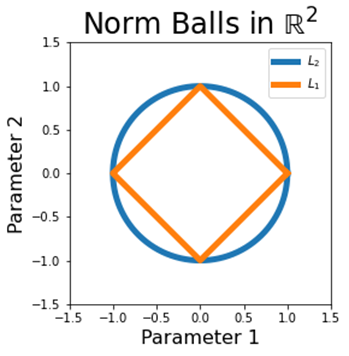
\includegraphics[width = 2.in]{balls.png}
\end{center}

We have a function $f(\vb x)$ that is constrained to $\norm{\vb x}_p \le k$ that we are hoping to minimize. We note that the constraint tells us
\begin{align*}
    \norm{\vb x}_p - k \le 0\qq{} \Rightarrow \qq{} \lambda\qty(\norm{\vb x}_p - k) = 0
\end{align*}
for some $\lambda$.
Our goal is to find 
\begin{align*}
    \argmin_{\vb x} f(\vb x) &=  \argmin_{\vb x} f(\vb x) + \lambda\qty(\norm{\vb x}_p - k) \\
    &= \argmin_{\vb x} f(\vb x) + \lambda\norm{\vb x}_p &\text{(since $-\lambda k$ only shifts function up or down)}
\end{align*}
and hence minimizing $f(\vb x)$ is equivalent to minimizing $f(\vb x) + \lambda \norm{\vb x}_p$. The $L_1$ norm gives sparser solutions because there are an infinite number of solutions in which one of the parameters can be zero whereas there is exactly one in the $L_2$ case.
\end{solution}
\newpage



\begin{problem}[Extra Credit]
\textbf{(Lasso)} Show that placing an equal zero-mean Laplace prior on each element of the weights $\thetab$
of a model is equivelent to $\ell_1$ regularization in the Maximum-a-Posteriori estimate
\begin{align*}
    \text{maximize: } & p(\thetab | \Dc) = \frac{p(\Dc | \thetab)p(\thetab)}{p(\Dc)}.
\end{align*}
Note the form of the Laplace distribution is
\[
    \mathrm{Lap}(x|\mu,b) = \frac{1}{2b}\exp\left(-\frac{|x-\mu|}{b}\right)
\]
where $\mu$ is the location parameter and $b>0$ controls the variance. Draw (by hand) and compare the density
$\mathrm{Lap}(x|0,1)$ and the standard normal $\Nc(x|0,1)$ and suggest why this would
lead to sparser solutions than a Gaussian prior on each elements of the weights
(which correspond to $\ell_2$ regularization).
\end{problem}
\begin{solution}
If we are hoping to maximize $p(\thetab | \Dc)$ then this is the same as asking to maximize the $\log p(\thetab | \Dc) $. And so
\begin{align*}
     \text{maximize: }  \log p(\thetab | \Dc) &= \log \frac{p(\Dc | \thetab)p(\thetab)}{p(\Dc)}= \log p(\Dc | \thetab) + \log p(\thetab) - \log p(\Dc)
\end{align*}
We ignore the constant term on the right. If we assume that $p(\thetab_i) \sim \mathrm{Lap}(\thetab_i|\mu=0,b)$, then 
\begin{align*}
    \log p(\thetab) &\propto \log \prod_i \mathrm{Lap}(\thetab_i|\mu=0,b)= \sum_i \log \mathrm{Lap}(\thetab_i|\mu=0,b) \\
    &=\sum_i \log\frac{1}{2b}\exp\left(-\frac{|\thetab_i|}{b}\right) \\
    &= - \sum_i\log 2b - \sum_i \frac{\abs{\thetab_i}}{b} \\
    &= - \sum_i\log 2b - \frac{1}{b}\norm{\thetab}_1
\end{align*}
This tells us that---if we ignore any constant terms---that maximizing $p(\thetab|\Dc)$ is the same as
\begin{align*}
    \text{maximize: }  \log p(\thetab | \Dc) &= \log p(\Dc | \thetab) - \lambda \norm{\thetab}_1 \qq{where} \lambda \equiv 1/b,
\end{align*}
or, equivalently,
\begin{align*}
    \text{minimize: }  \log p(\thetab | \Dc) &= -\log p(\Dc | \thetab) + \lambda \norm{\thetab}_1.
\end{align*}

Here is the plot comparing the Laplacian and Gaussian distributions (I'm sorry about the resolution):
\begin{center}
    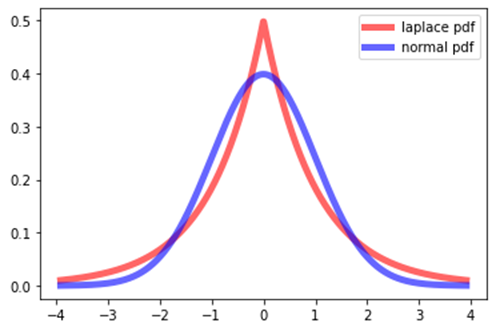
\includegraphics[width = 3.5in]{dist.png}
\end{center}
This would lead to sparser solutions presumably because more of the distribution is centered around zero than the Gaussian.
\end{solution}

\end{document}
